\documentclass[12pt, a4paper]{article}

\usepackage[utf8]{inputenc}
% Limit the page margin to only 1 inch.
\usepackage[margin=1in]{geometry}

%Imports biblatex package
\usepackage[
backend=biber,
style=alphabetic
]{biblatex}
\addbibresource{../../algs4e.bib}

% Enables the `align' environment.
\usepackage{amsmath}
% Provides useful environments, such as:
% - \begin{proof} ...\end{proof}
\usepackage{amsthm}
\usepackage[most]{tcolorbox}

\newtheorem*{proposition}{Proposition}

% Enables using \mathbb{}, for example \mathbb{N} for the set of natural numbers.
\usepackage{amssymb}

% Allows using letters in enumerate list environment. Use, for example:
%\begin{enumerate}[label=(\alph*)]
% ...
%\end{enumerate}
\usepackage[inline]{enumitem}

% Enable importing external graphic files and provides useful commannds, like \graphicspath{}
\usepackage{graphicx}
% Images are located in a directory called images in the current directory.
\graphicspath{{./images/}}

% Make links look better by default.
% See: https://tex.stackexchange.com/questions/823/remove-ugly-borders-around-clickable-cross-references-and-hyperlinks
\usepackage[hidelinks]{hyperref}
\usepackage{xcolor}
\hypersetup{
	colorlinks,
	linkcolor={red!50!black},
	citecolor={blue!50!black},
	urlcolor={blue!80!black}
}


% Code Listings. Source:
% https://stackoverflow.com/questions/3175105/inserting-code-in-this-latex-document-with-indentation
\usepackage{listings}
\usepackage{color}

\definecolor{dkgreen}{rgb}{0,0.6,0}
\definecolor{gray}{rgb}{0.5,0.5,0.5}
\definecolor{mauve}{rgb}{0.58,0,0.82}

\lstset{frame=tb,
	language=Java,
	aboveskip=3mm,
	belowskip=3mm,
	showstringspaces=false,
	columns=flexible,
	basicstyle={\small\ttfamily},
	numbers=none,
	numberstyle=\tiny\color{gray},
	keywordstyle=\color{blue},
	commentstyle=\color{dkgreen},
	stringstyle=\color{mauve},
	breaklines=true,
	breakatwhitespace=true,
	tabsize=3
}

\newcommand{\prob}{\text{P}}
%\newcommand{\complement}{\mathsf{c}}

% Define an environment called "ex" (for Exercise) so that I can do: \begin{ex}{1.5}...\end{ex}
\newenvironment{ex}[2][Exercise]
{\par\medskip\noindent \textbf{#1 #2.}}
{\medskip}

% Define a solution environment, similar to ex (exercise) environment.
\newenvironment{sol}[1][Solution]
{\par\medskip\noindent \textbf{#1.} }
{\medskip}

\begin{document}
	\noindent Sergio E. Garcia Tapia \hfill
	
	\noindent \emph{Algorithms} by Sedgewick and Wayne (4th edition) \cite{sedgewick_wayne}\hfill
	
	\noindent January 21, 2025\hfill 
	\section*{5.1: String Sorts}
	\begin{ex}{1}
		Develop a sort implementation that counts the number of different key values,
		the uses a symbol table to apply key-indexed counting to sort the array.
		(This method is \emph{not} for sure when the number of different keys is large).
	\end{ex}
	\begin{sol}
		It was unclear to me whether the sort implementation should allow for any type
		of key. I decided to limit the implementation to arrays of integers.
		
		See \texttt{com.segarciat.algs4.ch5.sec1.ex01}.
	\end{sol}
	\begin{ex}{2}
		Give a trace for LSD string sort for the keys:
		\begin{lstlisting}[language={}]
			no is th ti fo al go pe to co to th ai of th pa
		\end{lstlisting}
	\end{ex}
	\begin{sol}
		See Figure~\ref{fig:ex-02}.
		\begin{figure}
			\centering
			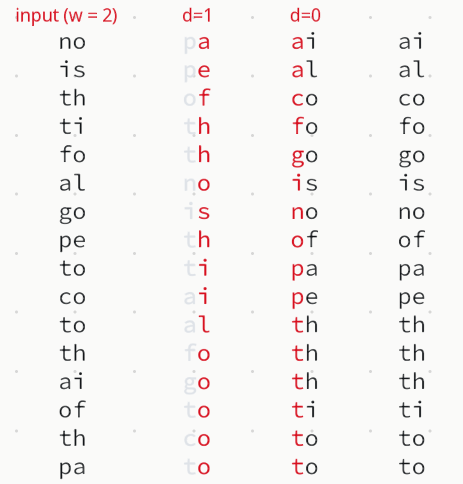
\includegraphics[width=0.4\textwidth]{exercise-02}
			\caption{Trace of LSD string sort for Exercise 2.}
			\label{fig:ex-02}
		\end{figure}
	\end{sol}
	\begin{ex}{3}
		Give a trace for MSD string sort for the keys
		\begin{lstlisting}[language={}]
			no is th ti fo al go pe to co to th ai of th pa
		\end{lstlisting}
	\end{ex}
	\begin{sol}
		See Figure~\ref{fig:ex-03}. The \texttt{CUTOFF} subarray length is \texttt{0} (no cutoff).
		Hence, we assume that insertion sort is used when the subarray is length 1, which
		would cause the method to immediately return anyway (because a 1-element array is sorted).
		Note that I omitted the recursive calls on singleton subarrays, such as the one containing
		\texttt{co}. I also omitted calls when the ends of the strings are reached because
		MST skips recursive calls on such strings.
		\begin{figure}
			\centering
			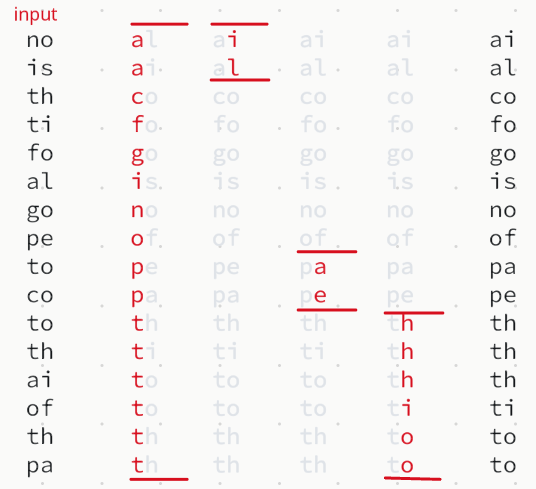
\includegraphics[width=0.4\textwidth]{exercise-03}
			\caption{Trace of MSD string sort for Exercise 3.}
			\label{fig:ex-03}
		\end{figure}
	\end{sol}
	\begin{ex}{4}
		Give a trace for 3-way string quicksort for the keys
		\begin{lstlisting}[language={}]
			no is th ti fo al go pe to co to th ai of th pa
		\end{lstlisting}
	\end{ex}
	\begin{sol}
		See Figure~\ref{fig:ex-04}.
		\begin{figure}
			\centering
			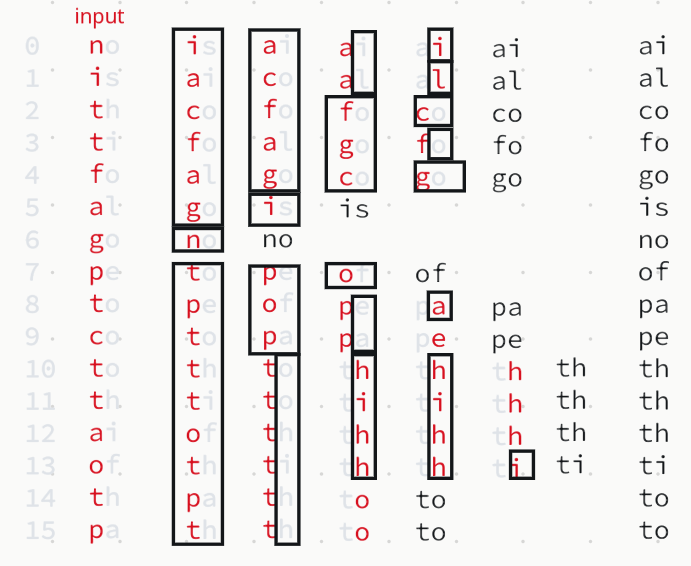
\includegraphics[width=0.4\textwidth]{exercise-04}
			\caption{Trace of 3-way string quicksort for Exercise 4.}
			\label{fig:ex-04}
		\end{figure}
	\end{sol}
	\begin{ex}{5}
		Give a trace for MSD string sort for the keys
		\begin{lstlisting}[language={}]
			now is the time for all good people to come to the aid of
		\end{lstlisting}
	\end{ex}
	\begin{sol}
		See Figure~\ref{fig:ex-05}.
		\begin{figure}
			\centering
			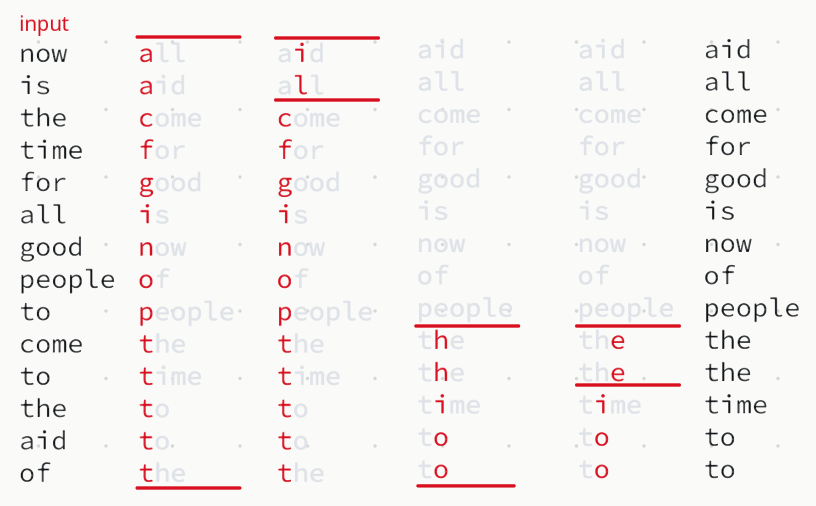
\includegraphics[width=0.5\textwidth]{exercise-05}
			\caption{Trace of MSD string sort for Exercise 5.}
			\label{fig:ex-05}
		\end{figure}
	\end{sol}
	\begin{ex}{7}
		Develop an implementation of key-indexed counting that makes use of an array
		of \texttt{Queue} objects.
	\end{ex}
	\begin{sol}
		See \texttt{com.segarciat.algs4.ch5.sec1.ex07}.
	\end{sol}
	\begin{ex}{8}
		Give the number of characters examined by MSD string sort and 3-way string quicksort
		for a file with $n$ keys \texttt{a}, \texttt{aa}, \texttt{aaa}, \texttt{aaaa},
		\texttt{aaaa}, $\ldots$
	\end{ex}
	\begin{sol}
		3-way string quicksort would require first $n$, then $n$ again, the $n-1$, and so on,
		which comes out to about $\Theta(n^2)$. That is, all characters are examined.
		
		Meanwhile, MSD would also examine all the characters. Unlike 3-way string quicksort,
		MSD would also incur the cost of initializing the \texttt{count} arrays, which
		it would do $nR$ times.
	\end{sol}
	\begin{ex}{9}
		Develop an implementation of LSD string sort that works for variable-length strings.
	\end{ex}
	\begin{sol}
		See \texttt{com.segarciat.algs4.ch5.sec1.ex09}.
	\end{sol}
	\begin{ex}{12}
		\emph{Alphabet}. Develop an implementation of the \texttt{Alphabet} API that is given
		on page 698 and use it to develop LSD and MSD sorts for general alphabets.
	\end{ex}
	\begin{sol}
		See \texttt{com.segarciat.algs4.ch5.sec1.ex12}.
	\end{sol}
	\pagebreak
	\printbibliography
\end{document}